\documentclass[10pt,twocolumn,letterpaper]{article}

\usepackage{cvpr}
\usepackage{times}
\usepackage{epsfig}
\usepackage{graphicx}
\usepackage{amsmath}
\usepackage{amssymb}
\usepackage{algpseudocode}% http://ctan.org/pkg/algorithmicx
\usepackage{algorithm}% http://ctan.org/pkg/algorithm
\usepackage{subfig} %for subfigure environment
\usepackage{multirow}
\usepackage{array}
\usepackage{url}
%\usepackage{bbm}


\usepackage[normalem]{ulem}

\newcommand{\argmax}{\operatornamewithlimits{argmax}}
\newcommand{\argmin}{\operatornamewithlimits{argmin}}
\newcommand{\eqdef}{\overset{\mathrm{def}}{=\joinrel=}}


% Include other packages here, before hyperref.

% If you comment hyperref and then uncomment it, you should delete
% egpaper.aux before re-running latex.  (Or just hit 'q' on the first latex
% run, let it finish, and you should be clear).
\usepackage[pagebackref=true,breaklinks=true,letterpaper=true,colorlinks,bookmarks=false]{hyperref}

\cvprfinalcopy % *** Uncomment this line for the final submission

\def\cvprPaperID{118} % *** Enter the CVPR Paper ID here
\def\httilde{\mbox{\tt\raisebox{-.5ex}{\symbol{126}}}}

% Pages are numbered in submission mode, and unnumbered in camera-ready
\ifcvprfinal\pagestyle{empty}\fi
\begin{document}

%%%%%%%%% TITLE
\title{Interactive Action Recognition from 3D Skeleton Data}

\author{Swami Sankaranarayanan, Kota Hara, Yiannis Aloimonos\\
Center for Automation Research, University of Maryland, College Park, MD 20742\\
{\tt\small \{swamiviv,kotahara\}@umiacs.umd.edu}
% For a paper whose authors are all at the same institution,
% omit the following lines up until the closing ``}''.
% Additional authors and addresses can be added with ``\and'',
% just like the second author.
% To save space, use either the email address or home page, not both
}


\maketitle
%\thispagestyle{empty}

%%%%%%%%% ABSTRACT
\begin{abstract}
In this work, we deal with the problem of recognizing actions that involve interaction between two people. For this purpose, we have created a dataset that involves ten different interactive actions using the Kinect Sensor. We extract discriminative features from the Skeleton data obtained from Kinect by extending the framework of \cite{Vemulapalli2013} to two person interactions. Further, we propose a Simultaneous Action detection and localization method using the Latent Structural SVM framework, where the latent variables are the start and end frames of an action in the given input video and the action category the video belongs too. We show both the effectiveness and limitations of our Feature Representation by directly applying simple multi-class classfication methods.
   
\end{abstract}

%%%%%%%%% BODY TEXT
\section{Introduction}
Human action recognition has been a major problem in computer vision community for many years. There are many applications of action recognition such as surveillance, health-care and human computer interaction. Most of the previous works focus on action recognition of a single person. The action classes considered in those works is limited to simple actions such as walking, running and jumping. 

There are several works which deal with action classes involved with multiple people. These classes are more complex to recognize than the single-person actions due to the complexity of the actions. The actions are defined not only by the motion of one person but also their interactive motions. We call these multiple-people actions as interactive actions.

The examples of interactive actions we consider in this work are exchanging objects and greetings between two people. For exchanging objects, we consider different types of the objects such as cards, a ball and a chair. Depending on the object being exchanged, their interactive movement come out in a different form. For greetings, we consider interactive actions such as shaking hands and bowing. Our goal is to recognize these different types of interactive actions from the 3d skeleton information.


Action recognition from the body skeleton information has been actively studied due to the advancement of motion capture systems such as Kinect. Typically the skeleton information is given in the form of 3d locations of a set of body joints. Many action recognition systems directly use these information as the input or convert the location information into a set of joint angles and then use them as the input. The focus of most of the previous research has been on the recognition part. 

\cite{Vemulapalli2013} proposed a new skeleton representation based on relative geometry across body parts that achieves state of art results on several standard single-person action recognition datasets. The benefit of their approach compared to the previously adopted skeleton representation is that their representation can directly capture the relationship between body parts that are not directly connected each other. Thus, it is more capable of recognizing actions in which the relationship between non-connected body parts, such as left arm and right arm, is more important. In this work, we extend \cite{Vemulapalli2013} to classify actions performed by two people.

%They compute the translation and rotation between each pair of body parts and map it to the tangent space to obtain a feature vector. 

For the recognition part, we develop an algorithm which not only predicts the action class but also localizes frames where actions are taking place. We perform this using two methods.
\begin{itemize}
\item In the first method, we use a heuristic Action Localization method described in Section 2. We extract the features on the localized frames and use popular techniques like SVM, K-nn and Classification trees in a mutli-class classification setting to get the action class labels. 
\item In the second method, we propose a Latent Structured SVM framework for localizing action and recognizing the action label. Specifically, we treat the staring and ending frames of the action as latent variables and jointly optimize the cost function in a max-margin manner. Note that this method does not require annotation for latent variables as they are automatically determined in the optimization process.
\end{itemize}
 In this work, we show the results only for the first method. The worl related to second method is under progress. 


The paper is organized as follows: Section 2 describes the proposed skeleton representation at each frame. Section 3 explains our heuristic action localization method. Section 4 presents the Joint Action Localization and Detection method that we propose, using a Latent Structural SVM framework. The comparison to some state-of-art approaches is done in Section 5. The Results are shown in Section 6, followed by Conclusion in Section 7.


\section{Heuristic Approach for Action Localization}\label{sec:actionlocalization}

The action sequences that are collected from the Kinect consists of several irrelevant frames which does not contain the action that we are looking for. Thus, given a video sequence it becomes important to approximately localize the action. This is a mandatory pre-processing step to extract realiable features that completely describe the action that  we are interested in. We alos assume throughout this work that there is only one continuous action that takes place throughout a given video sequence. In this section, we decribe a heuristic way to localize the action in a given video. A given video sequence consists of the following parts:
\begin{equation}
<Init. Action - Main Action - Finish>
\end{equation}
The heuristic described here tries to acquire the frames corresponding to the Main Action  in an automated way. We perform the localization in two steps:
\begin{itemize}
\item Computing the action center frames
\item Computing the start and end frames
\end{itemize}

The action center frame is computed as the frame where the distance between the interacting persons is the least. If there are multiple frames with the same distance value (this could occur since some interactions can last for a few frames), the action center frame is assigned as the minimum of those frames.

The start(end) of any interaction in the video could be implied by a constant decrease(increase) in distance between two persons. Thus, we compute the distance between the persons at each frame and identify when the rate of change of distance goes above(start) or below (end) a given threshold $\delta$, which is a user input parameter. 


As can be observed, this method does not yield us exact localization but an approximate one. In the subsequent section, we take care of this by imposing temporal smoothness on the features that we extract from each frame. 


\section{Skeleton Representation}\label{sec:Feat}

The underlying notion of using a Skeleton Representation for human actions is that the human motion can be represented as a set of rigid body motions, where the rigid bodies are the different body joints. The output from the Kinect sensor is 3d positions of 20 body joints for each person defined in the global coordinate. We define our skeleton representation for the first person as $S^{(1)}=(V^{(1)},E^{(1)})$, where $V^{(1)}=\{v_{1}^{(1)},v_{2}^{(1)},\dots,v_{N}^{(1)}\}, N=20$ denotes the set of joints and $E^{(1)}=\{e_{1}^{(1)},e_{2}^{(1)},\dots,e_{M}^{(1)}\}, M=19$ denotes the set of body parts ( See Fig.\ref{fig:skeleton}). Let $e_{m1}^{(1)},e_{m2}^{(1)} \in \mathcal{R}^3$ represents the starting and ending points of the body part $e_{m}^{(1)}$. Similarly we have $S^{(2)}=(V^{(2)},E^{(2)})$ for the second person.

First, we define the person specific local coordinate at the first person's shoulder center computed as $(v_5 + v_6)/2$ such that the x coordinate is aligned with the person's body orientation. Then we update both $S^{(1)}=(V^{(1)},E^{(1)})$ and $S^{(2)}=(V^{(2)},E^{(2)})$ using this new coordinates. This process makes our representation invariant to the global translation and orientation. 

Next we consider a set of body parts, $E=\{E^{(1)},E^{(2)}\}$, and for each pair of body parts $e_m$ and $e_n$, in $E$, we describe their relative geometry by the translation and rotation. The translation is computed as $T_{m,n}=e_{m1}-e_{n1}$. For the rotation, we compute the rotation axis $r$ and the rotation angle $\theta$ between two vectors $e_{n2}-e_{n1}$ and $e_{m2}-e_{m1}$. From them we compute a quaternion $q_{m,n} \in \mathcal{R}^4$ by $q_1=r_1 sin( \frac{\theta}{2} ), q_2=r_2 sin( \frac{\theta}{2} ), q_3=r_3 sin( \frac{\theta}{2}), q_4=cin( \frac{\theta}{2})$.

Thus, each pair of parts can be represented as 7 dimensional vector. Since there are $\binom{38}{2}$ such pairs, we have $\binom{38}{2} \times 7 = 4921$ dimensional vector. We do the same step by using the second person's local coordinate and concatenate two vectors to obtain the final feature vector representing two people configurations at a current frame.

\begin{figure}[htb]
\begin{center}
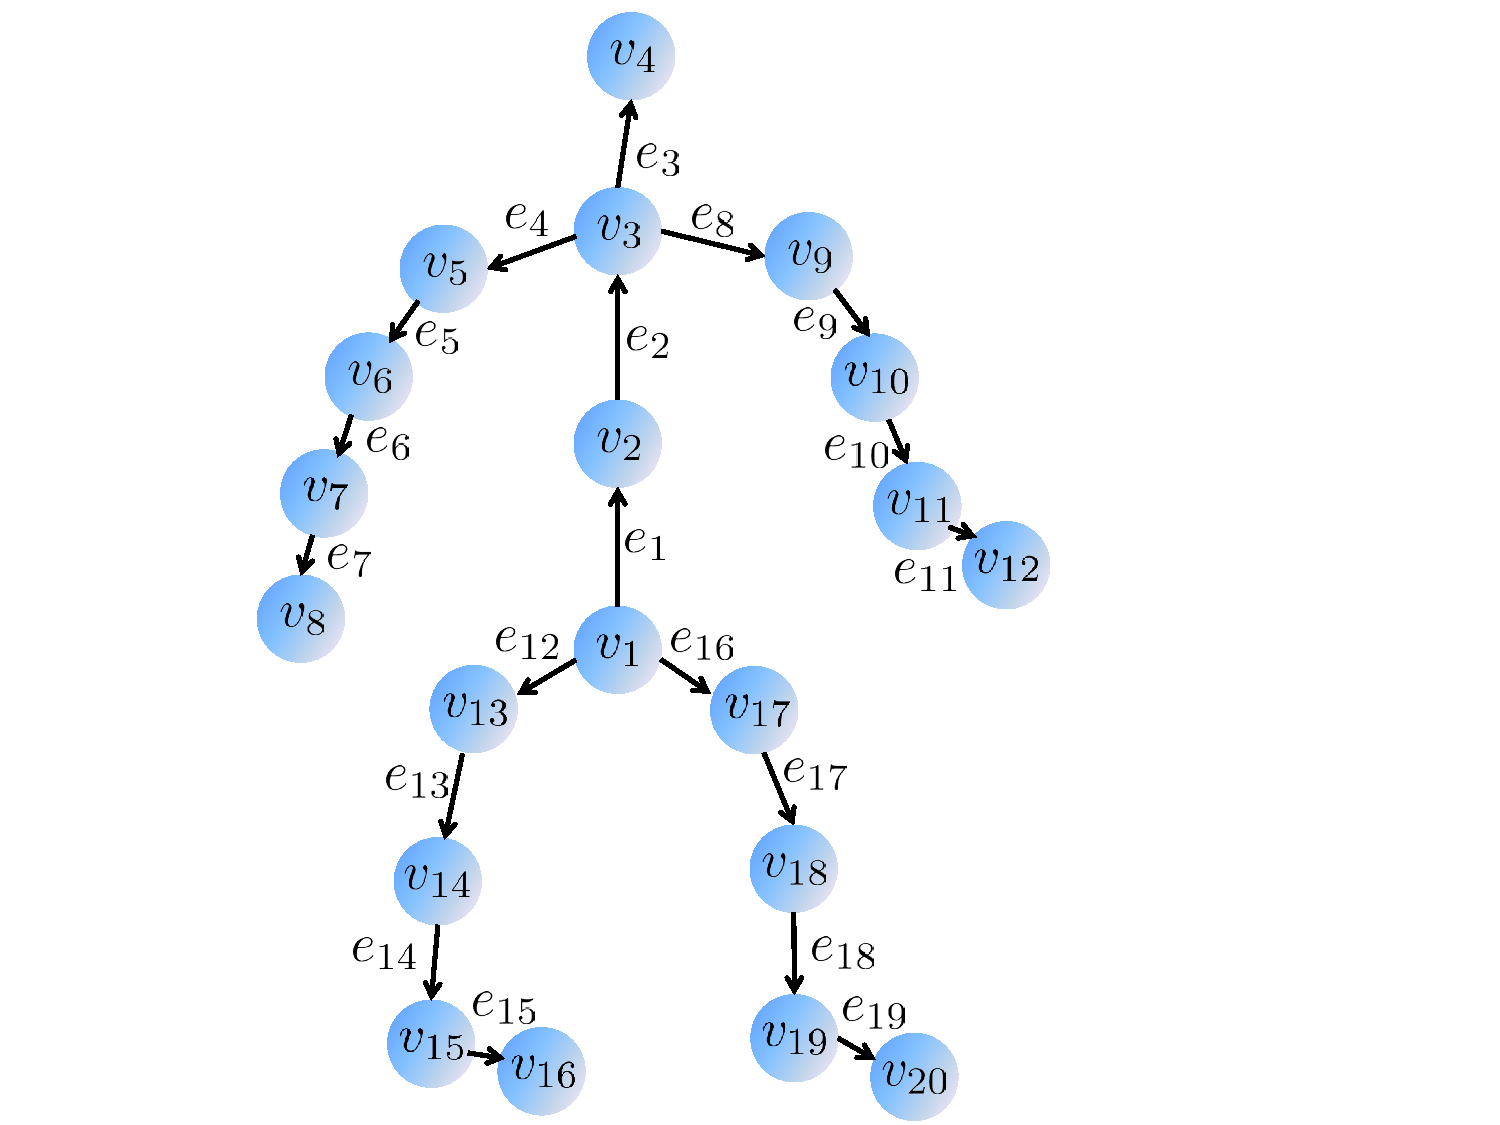
\includegraphics[width=2.3in]{skeleton.pdf}
\caption{An illustration of the skeleton. \label{fig:skeleton}}
\end{center}
\end{figure}

We compute our skeleton feature across 41 frames which includes the action center frame, 20 frames before the action center frame and 20 frames after the action center frame. Finally we concatenate all the feature vectors into a final vector.

%\section{Action Classification}
%We propose two different methods for classifying interactive actions from the skeleton features.
%
%\subsection{Generative Modeling}
%Given an input video containing the action, generate a semantic desription of the action as it occurs in the video. To describe an action would mean to generate a dictionary based representation for the action. A suitable middle ground between a complete linguistic action definition and a machine-derivable description, we borrow the action vocabulary decribed in \cite{SUHA}. Accordingly, a single person action in general can be described using an \textbf{operational triplet} as follows:
%
%\begin{equation}
%<Agent-Motion-Target>
%\end{equation}
%
%where $Agent$ is the person or the body part of the person which initiates the action; $Motion$ implies the movement of the $Agent$; $Target$ can be taken to be an object or another person or his body part that is involved in the interaction. Using this terminology some simple action representations can be generated as shown below:
%
%\begin{itemize}
%\item \textbf{Handshake}: $<$Arm1 - Outstretched - Arm2$>$
%\item \textbf{Kicking}: $<$Leg1 - Outstretched - Leg2$>$
%\end{itemize}
%
%It should be noted that for some actions that \textit{Agent} and \textit{Target} need not necessarily be a single person or body part but can be a collection of body parts that act on each other in a causal way. 
%\begin{figure}[ht]
%\centering
%
%  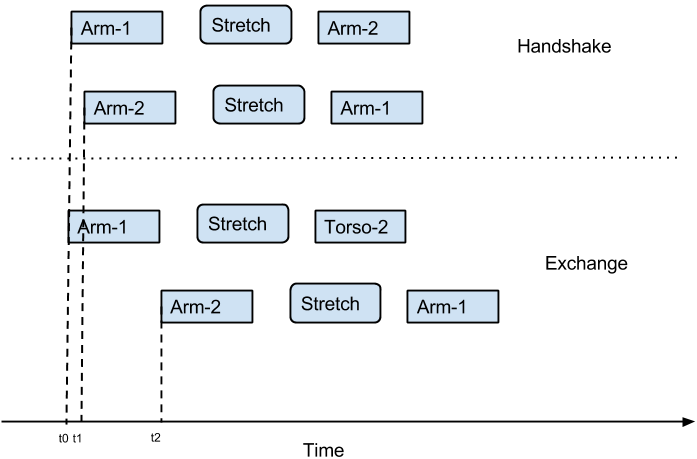
\includegraphics[scale = 0.3]{action_des.png}%
%  \label{Fig:act_des}%
%
%\end{figure}
%To see an example of this, consider the figure~\ref{Fig:act_des}. Thus, we can see that actions that have similar semantic descriptions in terms of the operational triplet can be differentiated by means of proper temporal constraints. 
%
%\begin{figure}[ht]
%\centering
%
%  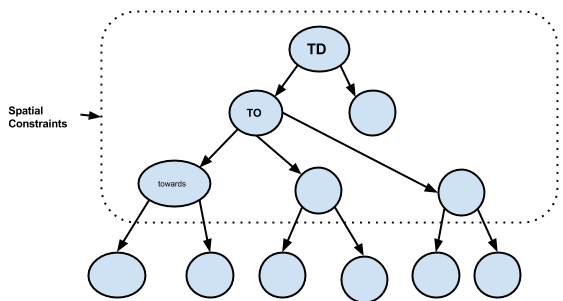
\includegraphics[scale = 0.3]{dec_tree.png}%
%  \label{Fig:tree}%
%
%\end{figure}
%
%<<<<<<< HEAD
%To look at how spatial constraints can decide the type of interaction, we incorporate that knowledge in the decision tree structure shown in figure~\ref{Fig:tree}.
%
%
%\subsection{Artificial Feed-forward Neural Network}
%We use artificial feed-forward neural network with softmax activation function as its final layer to estimate conditional probability, $P(y_t|x_t,t=t_{ac})$ at time instance $t$, where $y_t$ is an action class label and $x_t$ is the skeleton features computed from $t-20$ to $t+20$ frames and $t_{ac}$ is the time instance of the action center frame. We manually localize the action center frame of the training sequences and train the model with 10 hidden layers.
%=======
%\subsection{Artificial Feed-forward Neural Network}

%We use artificial feed-forward neural network with softmax activation function as its final layer to estimate conditional probability, $P(y_t|x_t,t=t_{ac})$ at time instance $t$, where $y_t$ is an action class label and $x_t$ is the skeleton features computed from $t-20$ to $t+20$ frames and $t_{ac}$ is the time instance of the action center frame. We manually localize the action center frame of the training sequences and train the model with 10 hidden layers.

%In testing time, we apply the trained neural network in a time sliding window manner and obtain the conditional probability $P(y_t|x_t,t=t_{ac})$. We also apply our action center detector at each frame to obtain $P(t=t_{ac}|x_t)$. We then compute $P(y_t,t=t_{ac}|x_t)=P(y_t|x_t,t=t_{ac}) P(t=t_{ac}|x_t)$ at each frame. Finally, we compute $P(y)$ for each sequence by $\sum_{t=t_{s}}^{t_{e}} P(y_t,t=t_{ac}|x_t)$ where $t_{s}$ and $t_{e}$ are the time instance where there are sufficient number of frames to apply the neural network. The final prediction is done by $\argmax_{y} P(y)$.

\section{Joint Action Localization and Classification}
In Sec.\ref{sec:actionlocalization}, we proposed a heuristic approach for action localization where the aim is to automatically determine when the action starts and ends. The problem of this approach is that it is not designed to achieve better classification accuracy. Also it is purely subjective to define the start and the end of the action.

Thus, we propose a method which can do both tasks simultaneously. In the proposed method, the training does not require manual labeling of the starting and ending frame of each action sequence. The model is trained in such a way that the starting and ending frame are determined in order to maximize the discriminativeness of the model. 

Our method is based on a latent structured SVM framework \cite{LatentSVM}. In this framework, we are given a set of training data
\begin{align*}
\mathcal{S}=\{(x_1,y_1),\dots,(x_N,y_N)\} \in (\mathcal{X},\mathcal{Y})^N
\end{align*},
where in our case, $x$ is skeleton feature extracted from a whole sequence and $y$ is an action class label.
Let $h$ denote a latent variable, which specifies the starting and ending frame of the sequence.

The prediction is done by finding $h$ and $y$ which maximize the following scoring function:
\begin{align}\label{eq:prediction}
f_{\mathbf{w}}(x) = \argmax_{(y,h) \in \mathcal{Y} \times \mathcal{H}} [ \mathbf{w} \cdot \Phi(x,y,h)]
\end{align}
where $\Phi(x,y,h)$ is a joint feature map. As a result, we not only obtain the predicted action class but also the starting and ending frame of the action in the given sequence.

In this work, we define the joint feature map $\Phi(x,y,h)$ as follows.
\begin{itemize}

  \item (Step 1) Extract part of $x$ between starting frame and ending frame (denoted as $\hat{x}$) 
  \item (Step 2) Expanding/Shrinking $\hat{x}$ by temporal resampling so that the dimensionality becomes a predefined number (denoted as $x^{*}$)
    \item  (Step 3) Setting $y$-th section of $\Phi$ as $x^{*}$ and remaining part as 0
\end{itemize}
\begin{equation}\label{M}
\Phi =
\begin{pmatrix}
  0  \\
  0  \\
  \vdots \\
  x^* \\
  \vdots \\
    0   \\
\end{pmatrix}
\in R^{ |\mathcal{Y}| \times dim(x^*)}
\end{equation}
The last step is a common approach taken for multiclass classification problems. This way, for each action class, different part of $\mathbf{w}$ is used and the class which has the highest score is chosen by Eq.\ref{eq:prediction}.

The training is done by solving the following optimization problem:
\begin{equation}\label{eq:optimization}
\begin{aligned}
\min_{\mathbf{w}} ||\mathbf{w} ||^2 + C \sum_{i=1}^{N} [ \max_{ (\tilde{y},\tilde{h}) \in (\mathcal{Y},\mathcal{H}) } [ \Delta(y_i, \tilde{y}) + \mathbf{w} \cdot \Phi(x_i, \tilde{y}, \tilde{h} )] - \\
\max_{h \in \mathcal{H}}  \mathbf{w} \cdot \Phi(x_i,y_i, h)]
\end{aligned}
\end{equation}
where $\Delta(y_i,y_j)$  is a loss function. We define the loss as
\[
  \Delta(y_i,y_j) = \begin{cases}
    0 & (y_i = y_j ) \\
    1 & (otherwise)
  \end{cases}
\]

By rewriting Eq.\ref{eq:optimization},
\begin{align*}\label{eq:optimization}
\min_{\mathbf{w}} ||\mathbf{w} ||^2 + C \sum_{i=1}^{N} [ \max_{ (\tilde{y},\tilde{h}) \in (\mathcal{Y},\mathcal{H}) } [ \Delta(y_i, \tilde{y}) + \mathbf{w} \cdot \Phi(x_i, \tilde{y}, \tilde{h} )]] - \\
C \sum_{i=1}^{N} [ \max_{h \in \mathcal{H}}  \mathbf{w} \cdot \Phi(x_i,y_i, h)]
\end{align*}
it is clear that the objective function is non-convex as it is defined as the difference between two convex function. We thus find a local optimum by EM-like algorithm where we first find, for each training sample, $h$ which maximize $\mathbf{w} \cdot \Phi(x_i,y_i, h)$. In our setting, this corresponds to finding the starting and ending frame for a training sample which make the score as high as possible.

In the second step, we fix $h$ and minimize $||\mathbf{w} ||^2 + C \sum_{i=1}^{N} [ \max_{ (\tilde{y},\tilde{h}) \in (\mathcal{Y},\mathcal{H}) } [ \Delta(y_i, \tilde{y}) + \mathbf{w} \cdot \Phi(x_i, \tilde{y}, \tilde{h} )]]$, which is convex. The maximization in the objective function corresponds to finding the most strict constrain for the optimization problem. To put it simply, we find a class $(\tilde{y}$ and $h$ where $(\tilde{y}$ is different from the true class but the score is high. 

The training is done by iteratively executing the above two steps while the decrease of the objective value becomes marginal.

Though we can use random values for the initial values for $h$, it is often desired to give a better initial values for $h$. We use the results of the heuristic approach described in Sec.\ref{sec:actionlocalization} as our initial values for $h$.

\section{Comparison to State-of-Art}
The problem of Action Recongition has been studied for different purposes by different communities including Computer Vision and Robotics. Most of the earlier approaches concentrate on recogizing Single Person Actions. Being a tough problem in its own right, the more interesting and informative actions are one that take place between a group of people. As a specific case, this work concentrates on Two-person interactions. There have been quite a few works that approach the same problem. These could be braodly divided into two categories: Semantic and Discriminative. An example of a Semantic approach is \cite{SUHA}, which builds a discriminative model by describing an action as an operational triplet : $<Agent-Motion-Target>$. They enumerate all possible combinations of the operational triplet in terms of different body parts and the different poses that they take. To impose temporal consistency, a dynamic Bayesian network is used and action classification is performed for each frame over a given video. Another work closest to the Action Localization decribed in the previous section is the Similarity Constrained Latent SVM, where they present an algorithm that learns from input videos that have action labels, and produces a classifier that can label test videos and mark a discriminative region of interest.

The novelty in our work comes from the fact that we extend the Skeleton Representation work of \cite{Vemulapalli2013} to two-person Interaction sequences. In our skeleton representation, in addition to the relative geometry across body parts within one person, we have also considered relative geometry between body parts across two people. We believe that this representation enables us to capture two person interactions well. For instance, our representation can capture the geometric relationship between a left arm of a person A and a right arm of a person B, which might be helpful to recognize the 'shaking hands' actions. The Latent SVM based approach that has been proposed in this work to perform Joint Action localization and Recognition has not been done previously for actions involving more than one person. 

\section{Experiments}

\subsection{Data Collection}

We create a new dataset named Maryland Interactive Action Dataset (MIAD) which consists of 10 interactive action classes captured by Kinect. The action classes we consider are summarized in Fig.\ref{fig:newactions} with their representative images. For each pair of people, we collect 2 sequences per an action class by switching their locations. Since we collect data from 6 pairs of people, there are 12 sequences per action class. We use the first X sequences as training data and the remaining sequences as testing data.

\begin{figure*}[htb]
\begin{center}
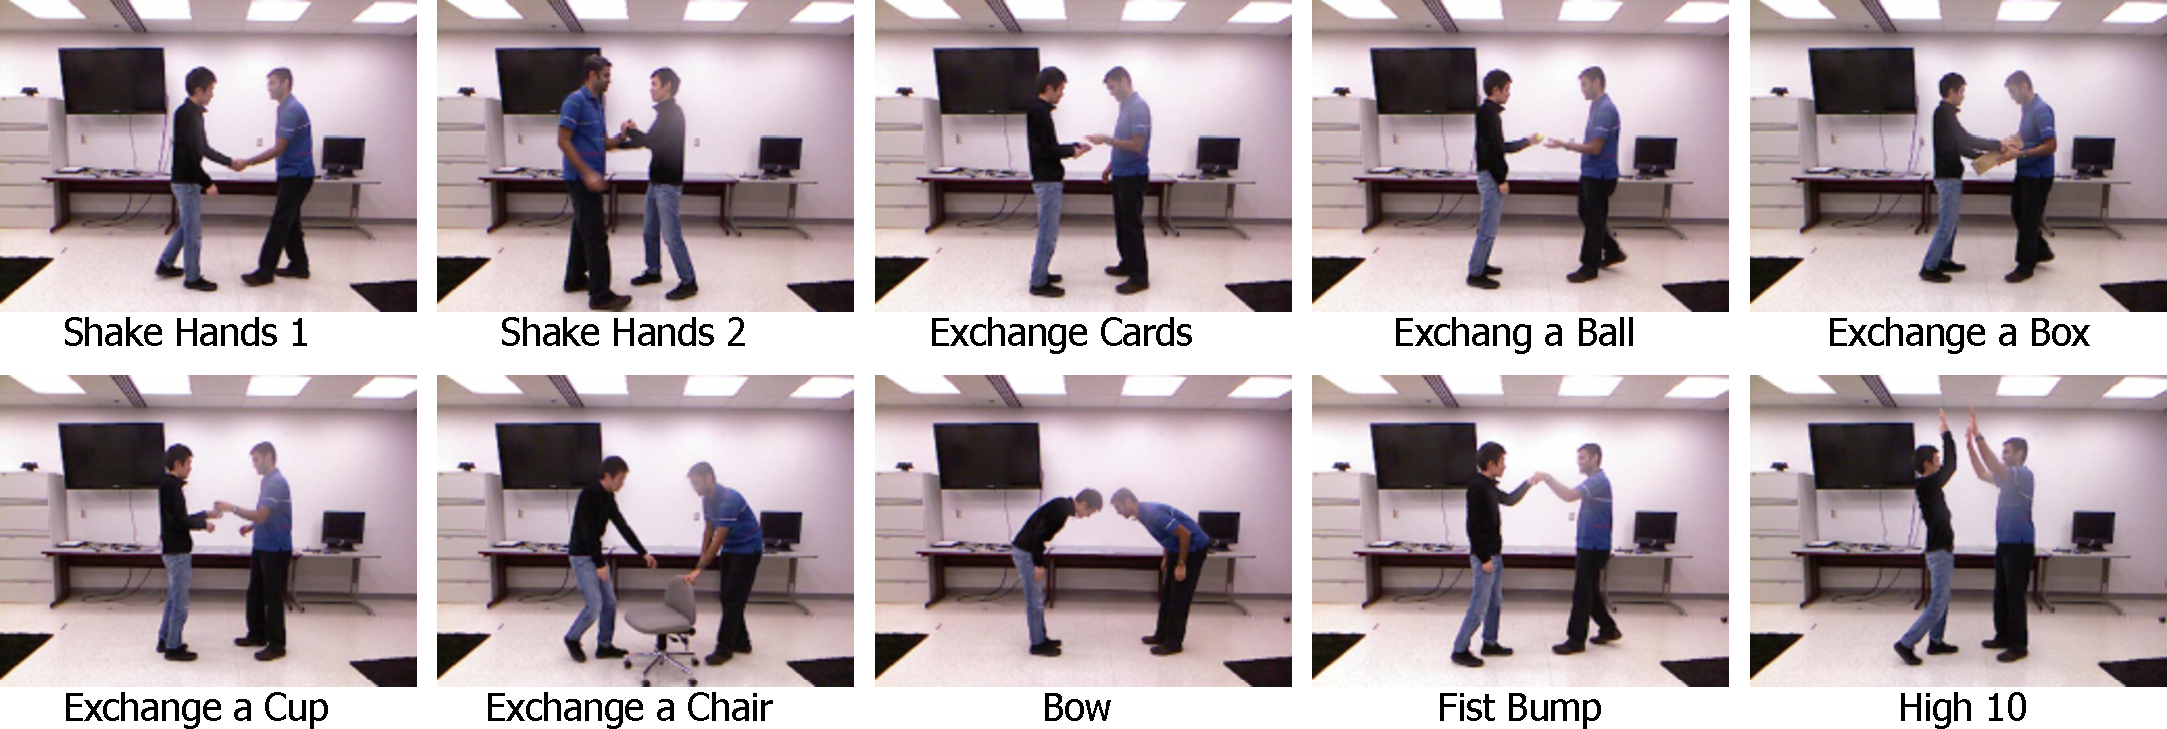
\includegraphics[width=6.8in]{newactions.pdf}
\caption{Action classes in newly collected MIAD dataset.  \label{fig:newactions}}
\end{center}
\end{figure*}

Our new data, MIAD differs from the existing two people interactive dataset such as K3HI \cite{K3HI} and SBU Kinect Interaction Dataset \cite{Yun2012}. First, our skeleton is represented by 20 joints whereas K3HI and SBU have only 15 joints. Second, the action classes we consider are more 'fine-grained'. In K3HI and SBU, there is only one action class for 'exchanging an object' class while MIAD contains 5 unique action classes for it, differentiated by the object being exchanged. Also K3HI and SBU have only one action class for the greeting action, namely, shaking hands, while MIAD includes 5 different action classes. These fine-grained actions are generally more challenging to discriminate as actions are more similar each other, necessitating more detailed representation of body movements.

%Steps for performing Interaction Recognition using Kinect:

%Step 0 : To organize the data in the above format. To do this, we extract skeleton data from the recorded OpenNI files that comes from the Kinect sensor.

%Step 1 : For each frame, we have to spatially localize each person - We are trying to figure out how to extract this information directly from the Kinect output

%Step 2 : Should perform an Object Detection routine to verify if there is any sign of Object exchange

%Step 3 : Based on how each joint moves in the video per frame, the activity trees are grown and the corresponding activity is detected. Primarily we want to differentiate between Object/Non-object Interactions and further classify the Non-Object Interactions into one of the Action classes that were given to us during Training. 

%The skeleton representation provides a convenient way to represent different actions in the form of Action trees. The terminal nodes of each action tree consists of the 20 joint positions. For each action, based on how different joint nodes combine to perform that action we can develop the corresponding action tree. 

\subsection{Action Localization Results}
In this section we show some sample results of our Action localization procedure described in Section~\ref{sec:act_local}. 
\begin{figure}[ht]

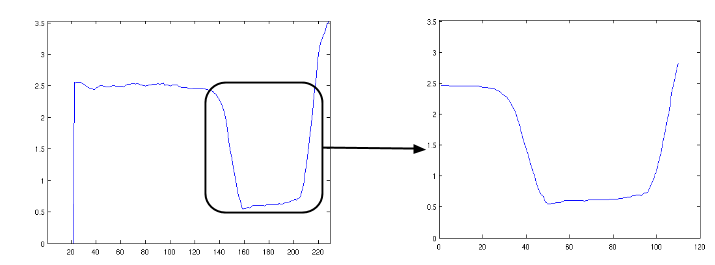
\includegraphics[scale=0.3]{act_local.png}
\caption{Distance Profile before(left) and after(right) localization}
\label{Fig:act_loc}

\end{figure}
Figure~\ref{Fig:act_loc} shows the difference in the distance profiles between the raw action sequence and the processed action sequence. As can be seen from Figure~\ref{Fig:act_loc}, the processed distance profile shows an appromiately zoomed in portion of the original profile. This localized region represents the frames in the given Video as to where the interaction takes place. 

\begin{figure}[ht]

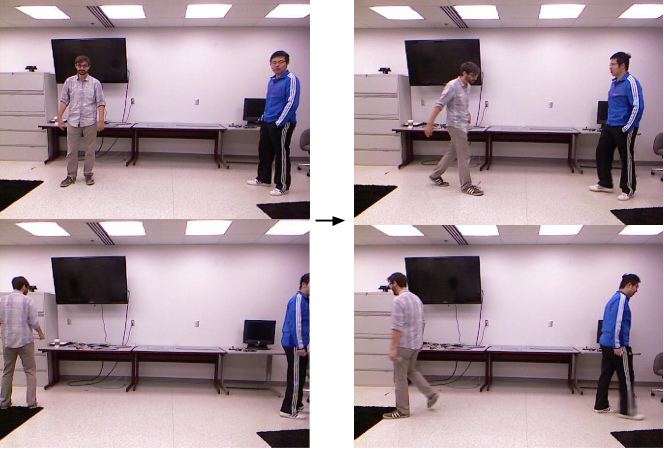
\includegraphics[scale=0.3]{first_last.png}
\caption{Start(Top) and End(Bottom) Frames}
\label{Fig:top_bot}
\end{figure}

Figure~\ref{Fig:top_bot} shows the start and end frames corresponding to the above action profiles. Thus, we use this simple heuristic method to extract only the relevant portion of the action sequence and provide this as input to our Feature extraction operator. 


\subsection{Action Classification Results}
To classify a given test input to one of the action classes, we learn a discriminative mapping between the input space and the output action label space. In the training stage, we learn the parameters of this mapping/classifier and apply them to classify the test input. In this work, we have used the following classification methods:
\begin{itemize}
\item Support Vector Machines (SVM): one (vs) one, one (vs) all 
\item k- Nearest Neighbour: k = 1,4
\item Classification Trees
\end{itemize}

SVM's are desgined to handle binary classification problems. To use them for multi-class classification, we use two paradigms which are explained as follows:
\begin{itemize}
\item \textbf{1(vs)1}: In this case, for each class combination $(i,j)$ one binary classifier is learnt. Thus for a $N$ class problem, the total number of classifiers becomes $\frac{N(N-1)}{2}$. 

\item \textbf{1(vs)all}: In this case, for each class $i$ in the training set, one classifier is learnt. The positive examples for this classifier are the inputs from class $i$ while the ngative examples are the rest of the inputs from all other classes. Thus, $N$ classifiers are learnt, one per class. 
\end{itemize}

Since SVM's produce only the decision values for a multi-class setting, we use Platt scaling as described in \cite{Platt1999} to convert these decision values to valid posterior probability estimates. Thus, for each classifier, for each test input $x_t$, we obtain the posterior probability measure $p(y=i|x_t)$, where $i$ is any class label between $\{1,10\}$ and assign that $i$  to $x_t$ which maximizes the probability measure. 
For each of these methods, we use different experimental settings by using different amounts of training and test data for each setting. The parameters for SVM are tuned using cross-validation  on the training set. 

\begin{table}[ht] 
\caption{Classification Accuracy} % title of Table 
\centering % used for centering table 
\begin{tabular}{c c c c c c} % centered columns (5 columns) 
\hline\hline %inserts double horizontal lines 
Split-Ratio  & SVM(1-1) & (1-all) & knn-1 & knn-4 & CT\\ [0.5ex] % inserts table 
%heading 
\hline % inserts single horizontal line 
20:80 &	18.4	 & 10.7  & 21.4 & 11.2 & 23.4 \\
40:60 &	17.4 &	23.2 & 26.1	& 18.8 &	 23.1 \\
60:40 &	26.5	 & 32.2	 & 32.7	& 20.4 &	 \textbf{28.6} \\
80:20 &	\textbf{40}   &	\textbf{51.8}	 & \textbf{40}	& \textbf{40}	   & 25 \\  [1ex]
\hline %inserts single line 
\end{tabular} 
\label{table:acc} % is used to refer this table in the text 
\end{table} 

\begin{figure}[ht]
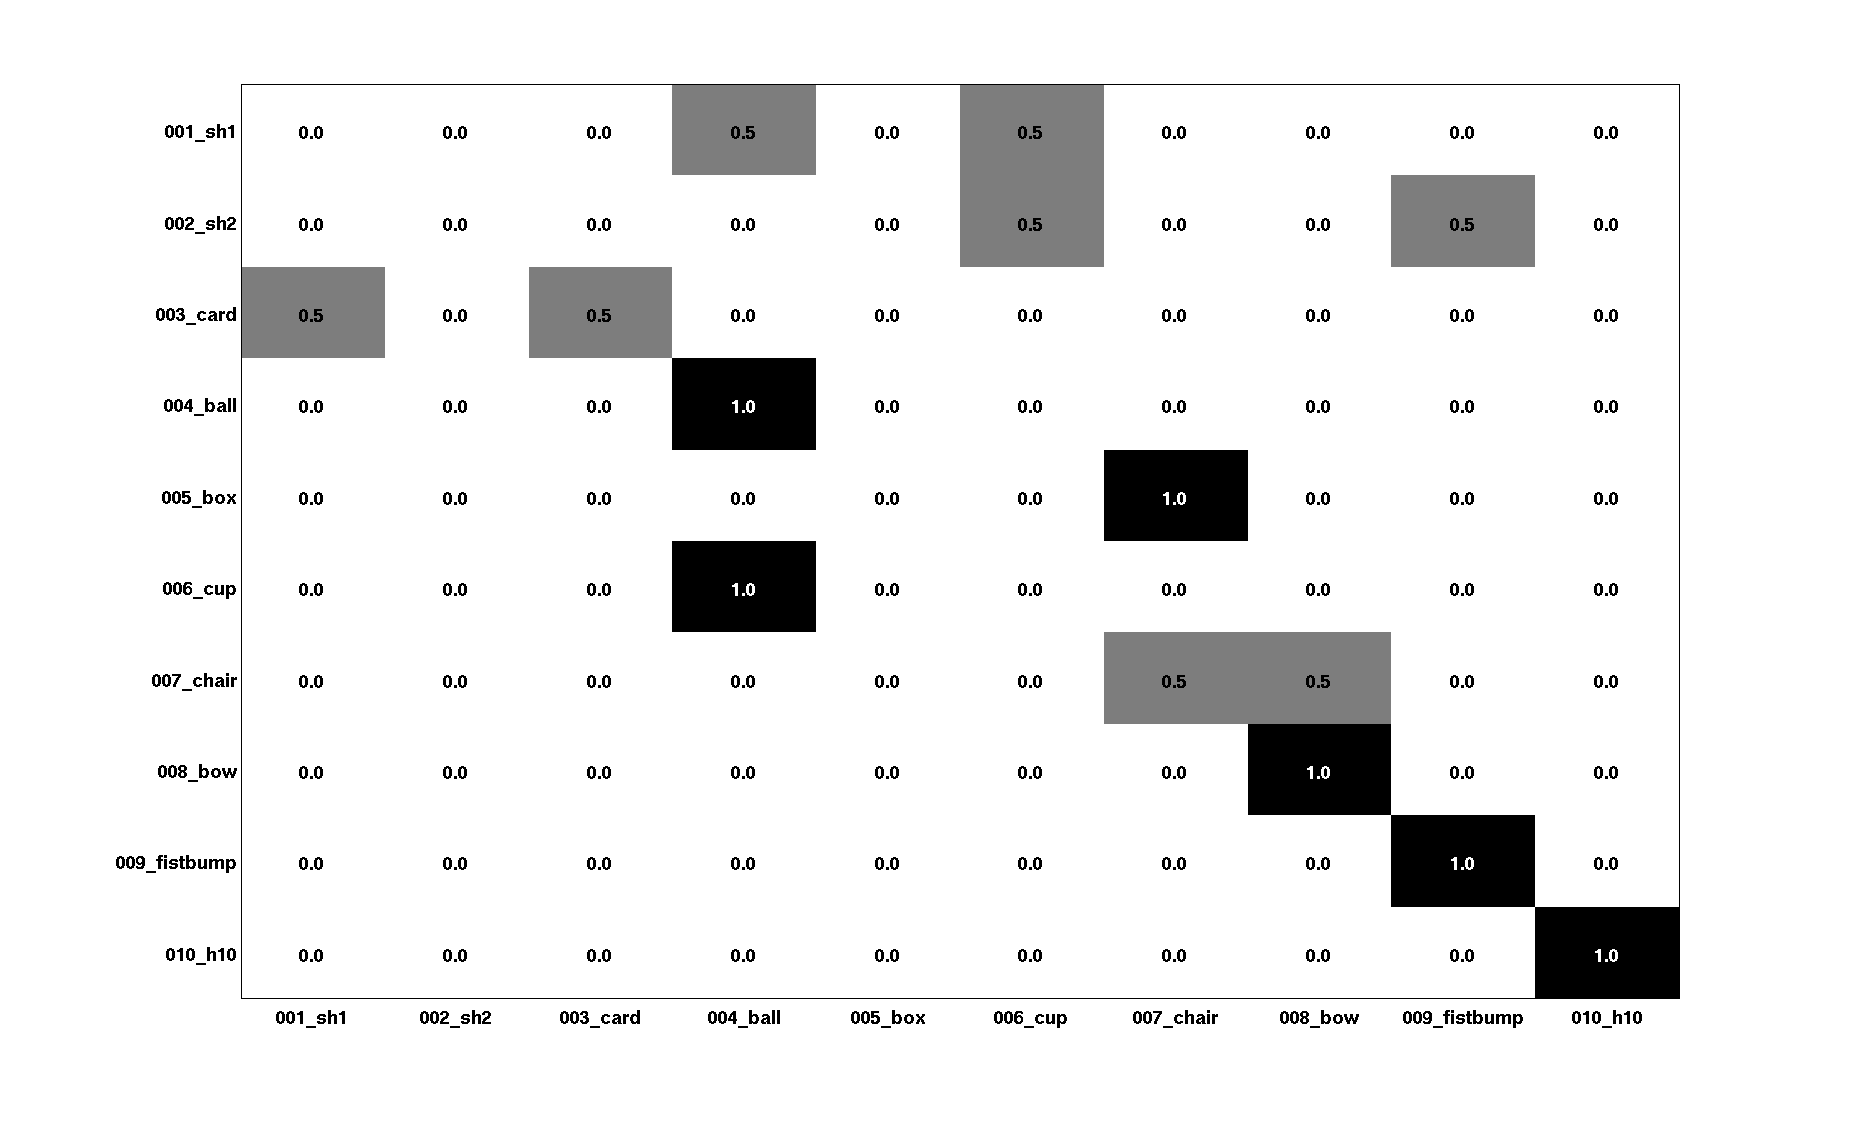
\includegraphics[scale=0.16]{conf_svm_ovr.png}
\caption{Confusion matrix for the best performing classification method (SVM one-vs-all). Darker color indicates larger values}
\label{Fig:conf_mat}
\end{figure}

\begin{figure}[ht]
\centering
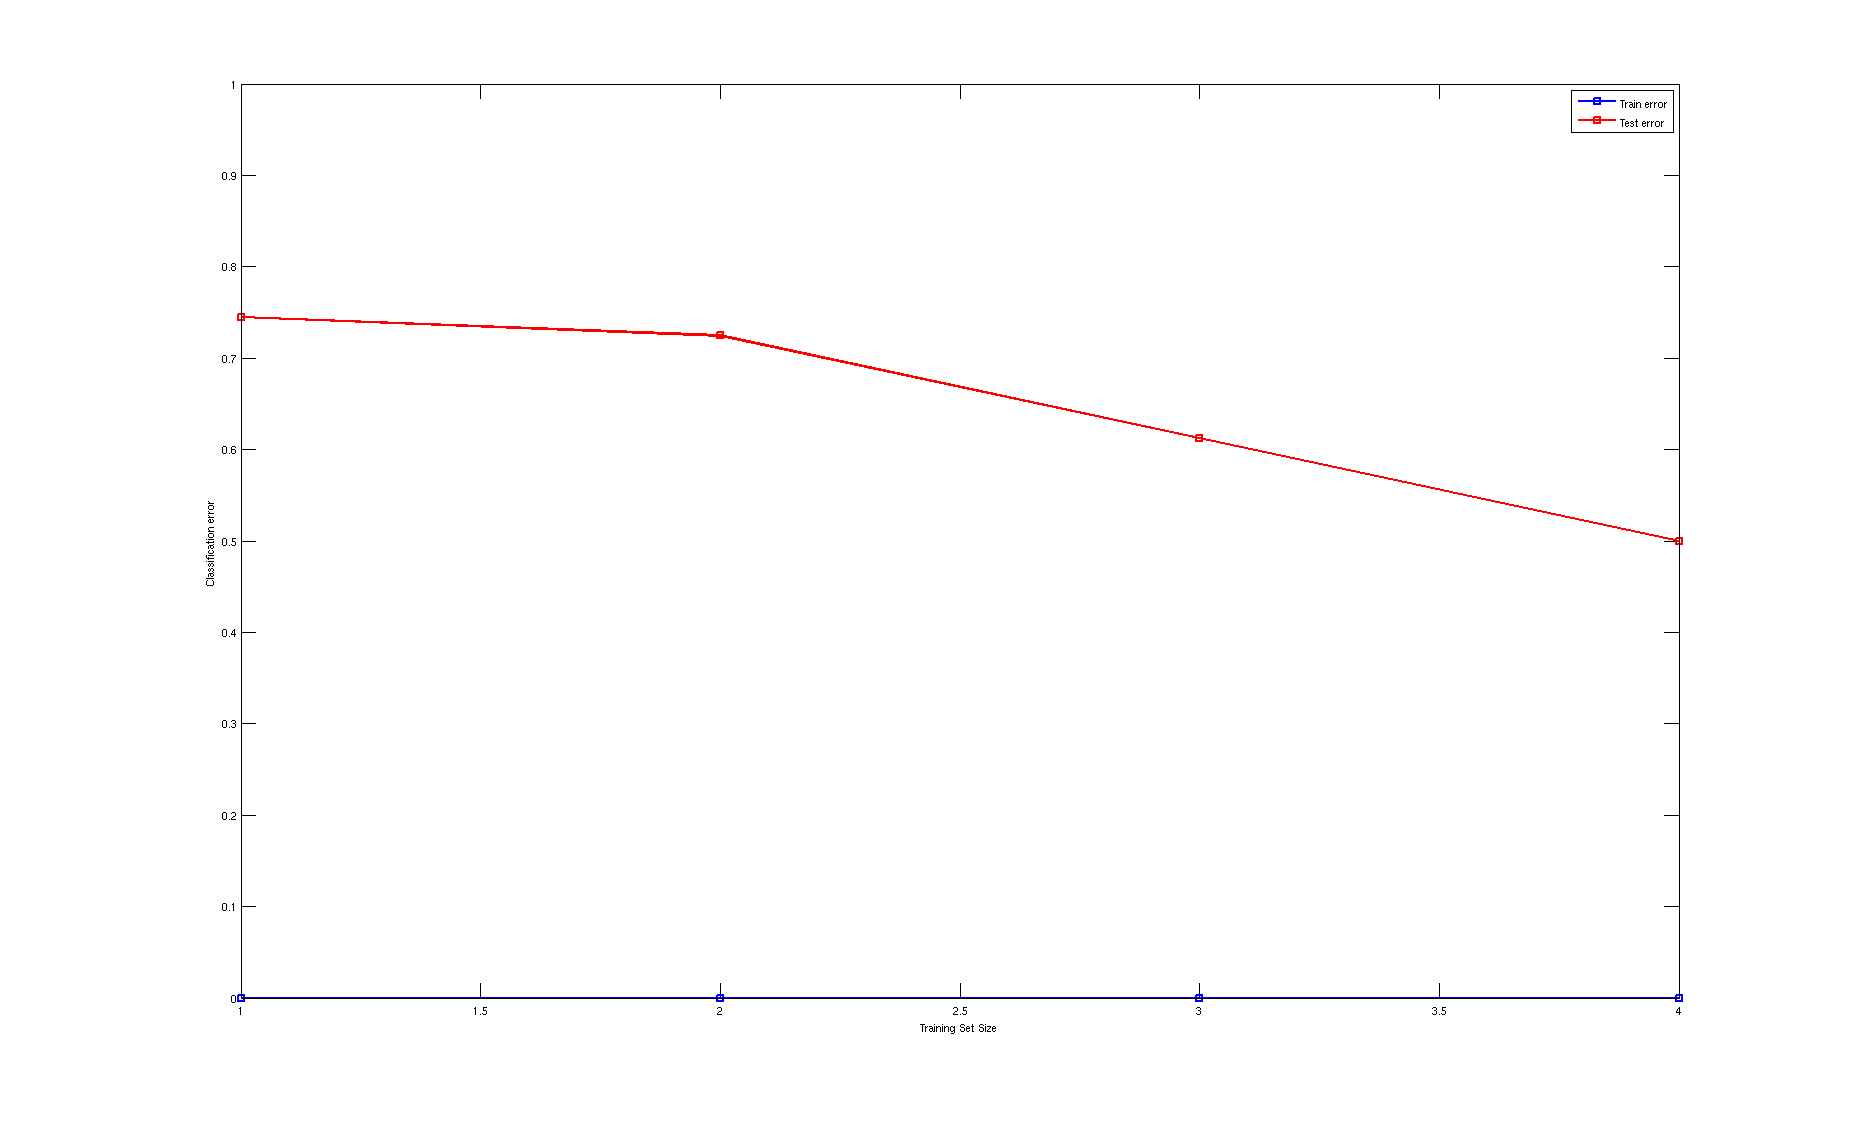
\includegraphics[scale=0.18]{svm_ovr_lc.png}
\caption{Learning Curve for SVM one-vs-all method}

\label{Fig:lc}
\end{figure}

The results for our classification method are shown in Table~\ref{table:acc}. Figure~\ref{Fig:conf_mat} shows the confusion matrix for the best performing classification method. The learning curve for the best performing classifier is shown in Figure~\ref{Fig:lc}.

\subsection*{Discussion}

\begin{figure}[ht]
\centering
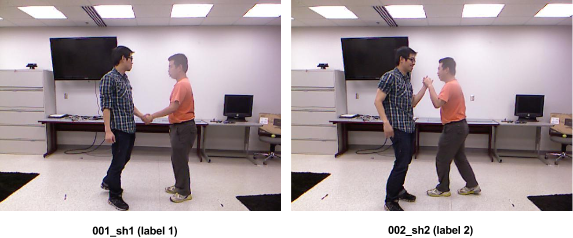
\includegraphics[scale=0.3]{sh_conf.png}
\caption{Variants of the shake hands action (Labels 1 and 2)}
\label{Fig:sh_conf}
\end{figure}
From the confusion matrix in Figure~\ref{Fig:conf_mat}, we can observe that the most confusing actions correspond to labels ${1,2}$ and ${5,6}$. Both labels ${1,2}$ correspond  to variations of the shaking hands action, one being the normal way and the other being an upright shake hands action. The scenario is shown in Figure~\ref{Fig:sh_conf}. Given that these actions are very difficult to distinguish and that different people perform these actions in different ways (such that the disriminative aspect is lost), the features extracted from the limited training data that we have could not clearly distinguish between these actions. 

Labels ${4,5,6}$ correspond to exchanging objects; box, ball and cup respectively. These could be more accurately classified by giving an additional information to the classifier involving the description of the object that appears in these frames. This part is a work under progress where we are trying to find an effective way to obtain an object description that would not be very computationally expensive. 
Furthermore, the learning curve in Figure~\ref{Fig:lc} shows that our model has very high variance, since the test error is much higher than the error on the training set. This implies that we can bridge the gap and thus improve the accuracy of our method by using more training data. 

\section{Conclusion}
In this work, we have attempted to classify Interactions involving two people. For this purpose, we have collected a database of Interactions that involve exchange of object and greeting actions. We have extended the existing state-of-art Skeleton representation technique to two-person Interaction sequences. The results were obtained by building a discriminative mapping between the action sequences and the action labels. We used several classifiers including SVM, k-nearest neighbour and Classification Trees. We demonstrated the limitations of such an approach given a minimal training dataset. We further hope to extend this work using the Latent-svm formulation to simultaneously detect and localize the action in an given input sequence. Furthermore, we are also exploring the use of attributes as a tool for classification, while also deriving suitable interpretation of an action sequence as would be described by a human. 

\begin{thebibliography}{9}

\bibitem{Vemulapalli2013}
  Raviteja  Vemulapalli,
  Felipe Arrate,
  Rama Chellappa,
  \emph{Human Action Recognition by Representing 3D Skeletons as Points in a Lie Group}.
  CVPR,
  2014.

\bibitem{SUHA} Semantic-level Understanding of Human Actions and Interactions using Event Hierarchy, Sangho Park, J.K. Aggarwal, CVPR'04

\bibitem{K3HI}
	Sangho Park,
	J.K. Aggarwal,
	\emph{K3HI: Kinect-based 3D Human Interaction Dataset}

\bibitem{Yun2012}
	Kiwon Yun, Jean Honorio, Debaleena Chattopadhyay, Tamara L. Berg, and Dimitris Samaras,
	\emph{Two-person Interaction Detection Using Body-Pose Features and Multiple Instance Learning}.
	CVPRW,
	2012.
	
	\bibitem{Platt1999}
	John C. Platt,
	\emph{Probabilistic Outputs for Support Vector Machines and Comparisons to Regularized Likelihood Methods}.
	ADVANCES IN LARGE MARGIN CLASSIFIERS, MIT Press, 1999.
	 
	

\bibitem{LatentSVM} Learning structural SVMs with latent variables, Chun-Nam John Yu and Thorsten Joachims, ICML'09.



\end{thebibliography}

\end{document}
